\chapter{Data preparation} \label{ch:data_preparation}

The third phase of the CRISP-DM process model for data mining projects is data preparation;
this chapter discusses the steps taken to implement the spatial and temporal relationships between the different data sources combined into the GTHA housing market database;
the nature of these relationships was discussed in chapter~\ref{ch:spatial_and_temporal_relationships}.
In addition, this chapter introduces new features derived from native Teranet attributes for land use classification, which will be described in chapters~\ref{ch:ml_workflow} and~\ref{ch:model_evaluation}.

The ``wicked'' nature of transportation and land use interaction introduced in chapter~\ref{ch:background} dictates the need to iteratively ``re-solve'' transportation and land use planning problems instead of focusing on finding some single ``optimal solution''.
This approach resembles the methodologies typically employed for data science projects, where the sequence of steps is iterated over, producing a more meaningful solution on each new iteration of the cycle, as defined by such process models as CRISP-DM\cite{Shearer2000}.
Similarly, data preparation can be followed in a linear manner, but is very likely to be iterative in nature\cite{Brownlee2013}.

\vspace{5mm}

Data preparation plays a critical role in research projects:

\begin{itemize}
    \item it is a prerequisite for any meaningful analysis
    \item data quality and the amount of useful information that it contains can determine the success of application of machine learning algorithms\cite{RaschkaMirjalili2017}
    \item it is often required to allow the introduction of constraints necessary for implementation of RDBMS
\end{itemize}

\vspace{5mm}

To facilitate easy modification and replication of the data preparation process for data sources related to the GTHA housing market database, a streamlined data preparation workflow using Python via a series of jupyter notebooks has been established as a part of this master's thesis.
It accomplishes three main objectives:
\begin{itemize}
    \item Clean Teranet dataset and correct its records for consistency.
    \item Introduce new keys that would allow efficient joining of other data sources, such as Census and TTS variables or parcel-level land use information, while maintaining the integrity of spatial and temporal relationships that were discussed in chapter~\ref{ch:spatial_and_temporal_relationships}.
    \item Engineer the new features that can be used by the machine learning algorithm along with the features from the joined datasets to classify land use, which will be discussed in chapters~\ref{ch:ml_workflow} and~\ref{ch:model_evaluation}.
\end{itemize}

This chapter introduces the concepts of ``Tidy Data'' and database normalization and outlines the standardized data preparation workflow that was designed to implement the spatio-temporal relationships discussed in chapter~\ref{ch:spatial_and_temporal_relationships} for all data sources that were combined into the GTHA housing market database that was implemented as a part of this master's thesis.

\section{Tidy data and database normalization} \label{sec:db_norm_tidy_data}

Hadley Wickham in his paper ``Tidy Data''\cite{Wickham2014} formalized the way in which a shape of the data can be described and what goal should be pursued when formatting data.
The ``tidy data'' standard is closely related to Edgar F. Codd's relational algebra and has been designed to facilitate initial exploration and analysis of the data, and to simplify the development of data analysis tools that work well together.
As an integral part of his relational model, Codd\cite{Codd1990} proposed a process of database normalization, or restructuring of a relational database in accordance with a series of so-called normal forms in order to reduce data redundancy and improve data integrity.
Normalization entails organizing the columns (attributes) and tables (relations) of a database to ensure that their dependencies are properly enforced by database integrity constraints.
The principles of ``tidy data'' formulated by Wickham essentially reformulate Codd's ideas in statistical language.

According to Wickham\cite{Wickham2014}, ``tidy data'' is a standard way of mapping the meaning of a dataset to its structure.
A dataset is ``messy'' or ``tidy'' depending on how rows, columns and tables are matched up with observations, variables and types.

\vspace{5mm}

In ``tidy data'':
\begin{enumerate}
    \item Each variable forms a column.
    \item Each observation forms a row.
    \item Each type of observational unit forms a table.
\end{enumerate}

This definition of ``tidy data'' matches Codd's 3rd normal form\cite{Codd1990}, but with the constraints framed in statistical language, and the focus put on a single dataset rather than on many connected datasets common in relational databases.
``Messy data'' is any other arrangement of data.

\vspace{5mm}

The structure of Teranet's dataset conforms with the ``tidy data'' format.
Contrary to Teranet, tables with select Census and TTS variables had variables for different Census and TTS years recorded as columns.
This needed to be addressed by unpivoting these tables and introducing a new attribute `year' to be used as a part of a composite foreign key when joining these variables with Teranet records;
thus, both spatial and temporal relationships that were introduced in chapter~\ref{ch:spatial_and_temporal_relationships} can be respected when combining these data sources together.

\vspace{5mm}

Tables with select Census and TTS variables were unpivoted to conform with the ``tidy data'' format:
\begin{itemize}
    \item each Census / TTS variable now forms a single column
    \item each value of Census / TTS variables is indexed by a composite primary key constituting of its spatial identifier (`DAUID' or `TAZ\_O', introduced in chapter~\ref{ch:spatial_and_temporal_relationships}) and the year of the survey
\end{itemize}

Introduction of the new foreign keys to Teranet records is described in the following section.

\section{Introduction of new keys and attributes via spatial and temporal relationships} \label{sec:introduction_of_new_keys}

To implement the spatial and temporal relationships between the data sources discussed in chapter~\ref{ch:spatial_and_temporal_relationships}, a number of new foreign keys needed to be introduced to Teranet records.
The new foreign keys either represent spatial identifiers (such as `dauid' or `taz\_o', corresponding to DA or TAZ within which a Teranet record is located), or an attribute identifying the year of Census or TTS survey, variables from which can be joined with this Teranet record.
Foreign keys representing spatial identifiers were added via a series of spatial joins while foreign keys identifying temporal spans were generated based on temporal spans defined earlier.

\vspace{5mm}

New spatial identifiers were introduced to each Teranet record via a series of spatial joins:
\begin{enumerate}
    \item 9,039,241 Teranet points were joined with 9,182 polygons of Dissemination Areas (DAs) for GTHA used by Census variables
    \begin{itemize}
        \item Teranet records with coordinates falling outside of GTHA boundary were filtered out
        \item From the original 9,039,241 records, 6,803,691 remained in the dataset
        \item New foreign keys `dauid', `csduid' and attribute `csdname' were added to each Teranet record
    \end{itemize}
    \item 6,803,691 Teranet points were joined with 1,716 polygons of Traffic Analysis Zones (TAZ) used by TTS variables
    \begin{itemize}
        \item New foreign key `taz\_o' was added to each Teranet record
    \end{itemize}
    \item 6,803,691 Teranet points were joined with 525 polygons of Forward Sortation Areas (FSA) and 555,668 polygons of postal geography from DMTI's Platinum Postal Geography Suite
    \begin{itemize}
        \item New foreign keys `fsa' and `pca\_id' and attribute `postal\_code\_dmti' were added to each Teranet record
        \item These keys are not currently used for joining any variables, but were added to expand the potential for relating datasets, as might be needed for the Longitudinal Housing Market Research conducted by UTTRI, which was introduced in section~\ref{sec:longitudinal_housing_market_research}
    \end{itemize}
    \item 6,803,691 Teranet points were joined with 1,664,862 polygons of parcel-level detailed land use provided by the Department of Geography
    \begin{itemize}
        \item New foreign keys `pin\_lu', `landuse' and `prop\_code' were added to each Teranet record
        \item Foreign keys `landuse' and `prop\_code' are codes that can be converted to land use categories that were used by the Department of Geography for GTA and Hamilton, respectively
        \item For records from Hamilton, `prop\_code' was converted to categories used by GTA land use and reassigned to `landuse', bringing GTA and Hamilton records to a single system of land use categories
    \end{itemize}
    \item Subsets of Teranet points were joined with corresponding yearly polygons of parcel-level land use from DMTI
    \begin{itemize}
        \item New attribute `dmti\_lu' was added to each Teranet record
    \end{itemize}
\end{enumerate}

\begin{figure}[hbt!]
    \centering
    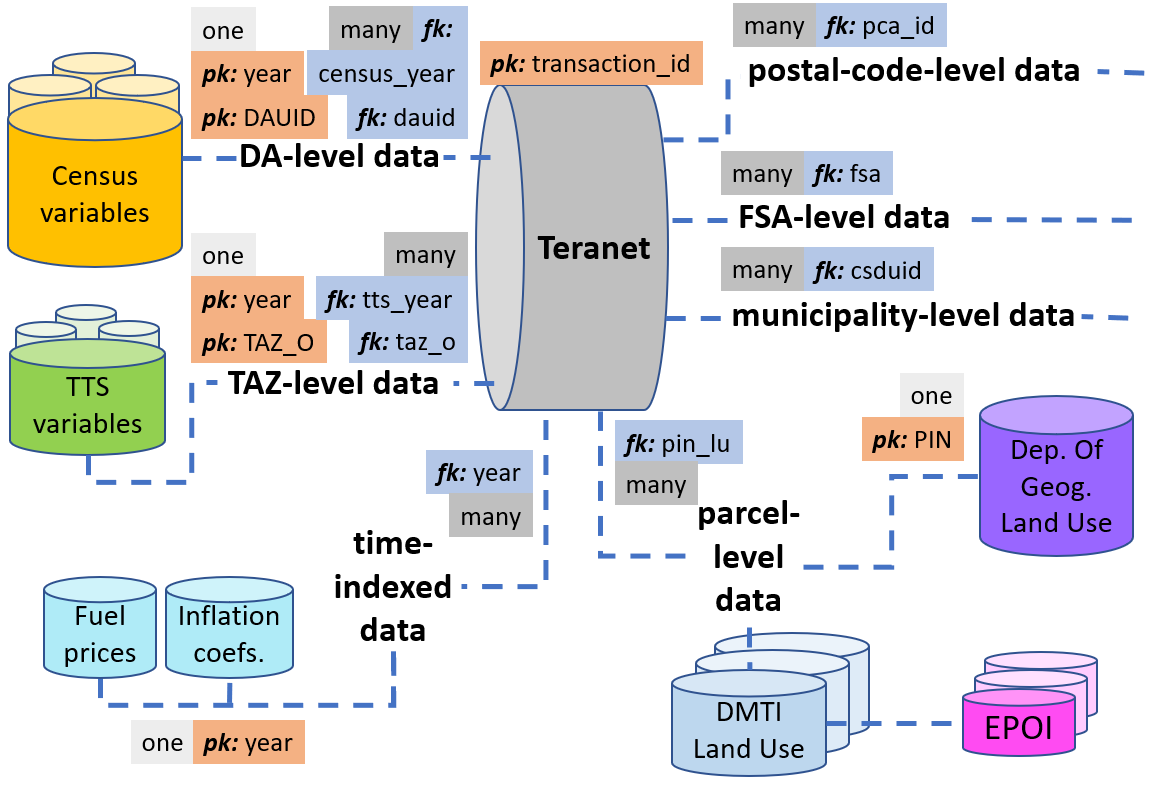
\includegraphics[width=1\linewidth,trim=0 0 0 0,clip]{data_relations.png}
    \caption{Relationships between datasets introduced during data preparation were then used to set up referential integrity constraints of the new PostgreSQL database for GTHA housing market data.
    The Entity Relationship (ER) diagram for the database created as a part of this thesis can be found in Appendix~\ref{ch:appendix_rdbms};
    its referential integrity constraints were implemented based on the spatial and temporal relationships between data sources that were introduced in chapter~\ref{ch:spatial_and_temporal_relationships}.}
    \label{fig:data_relations}
\end{figure}

Foreign keys representing temporal identifiers used for matching Teranet records with Census / TTS variables were generated from the registration date of each Teranet record, matching each year of Teranet records with a corresponding 5-year span covered by a Census or TTS survey, as was discussed in section~\ref{sec:termporal_relationships_between_datasets}.
Diagram of relationships that were introduced between datasets for the implementation of RDBMS and their primary and foreign keys is presented on figure~\ref{fig:data_relations}.

Following the steps described above ensures that the integrity of spatial and temporal relationships is maintained when combining attributes from different data sources at Teranet transaction level, as required by the Longitudinal Housing Market Research conducted by UTTRI, which was introduced in section~\ref{sec:longitudinal_housing_market_research}.
For example, Teranet records from 2007 would be spatially joined with DMTI land use data from 2007, and are matched by their attributes `census\_year' and `tts\_year' to Census and TTS variables from 2006 Census and TTS surveys.
Census and TTS variables can be joined by appropriate `dauid' and `taz\_o' (composite foreign keys are used when joining), and thus all data sources can be spatially and temporally aligned at the level of Teranet transactions.

Typically, a database table has an attribute, or a combination of multiple attributes, whose values are unique across the whole table;
minimal combinations of attributes allowing unique identification of records are also referred to as candidate keys.
Primary keys, chosen from candidate keys, are one of the most important concepts in database design.
Almost every database table should have a primary key, chosen from a set of candidate keys.
The main purpose of a primary key is to uniquely identify records in a table, and ideally, primary keys are determined using as few columns as possible.

In case of Teranet records, no combination of columns constitutes a candidate key, as it is possible to have two valid Teranet records that have duplicated values across all native features.
For example, two same-price condo units sold in the same building on the same day can have duplicated values across all the native Teranet features.
Such a scenario is not impossible since condo sales often come in large batches of sales over a short period of time;
and in some cases, all records from a building are recorded under a single `pin'.

To address this, a new surrogate key (artificial unique identifier for RDBMS) was added to each Teranet record via a new attribute `transaction\_id'.
With this new attribute, Teranet's dataset can fit into a normalized database using the new attribute `transaction\_id' as its primary key.
As was discussed in section~\ref{sec:db_norm_tidy_data}, the unpivoted tables with select Census and TTS variables have composite primary keys consisting of a unique spatial identifier (`DAUID' or `TAZ\_O', respectively) and the year of the survey.
Thus, semantic interoperability can be ensured when joining variables from these sources at the Teranet transaction level.
Relationships introduced via the operations described in this section formulate referential integrity constraints that have been used to set up a PostgreSQL database of GTHA housing market data;
its Entity Relationship (ER) diagram can be found in Appendix~\ref{ch:appendix_rdbms}.

\section{Outliers} \label{sec:outliers}

Outliers present an issue for machine learning as they lead to difficulties in visualizing data and, more importantly, can degrade the predictive performance of an algorithm.
In addition, outliers, if left unscaled, can significantly slow down or even prevent the convergence of many gradient-based algorithms, such as Logistic Regression\cite{Scikit-learndevelopers2019b}.
However, an exact definition of what constitutes on outlier within a given dataset presents a challenge in itself, since it depends on hidden assumptions regarding the data structure and the applied detection method\cite{Ben-Gal2005}.
As defined by Hawkins, an outlier is an observation that deviates so much from other observations as to arouse suspicion that it was generated by a different mechanism\cite{Hawkins1980}.

\begin{figure}[ht]
    \centering
    \begin{subfigure}{\linewidth}
        \centering
        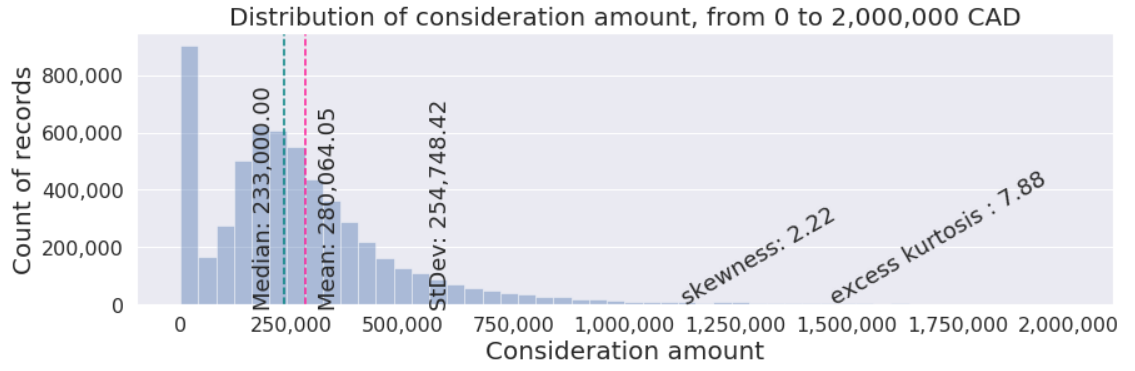
\includegraphics[width=.95\linewidth]{price_dist_raw.png}
        \caption{From 0 to 2,000,000 CAD}
    \end{subfigure}

    \begin{subfigure}{\linewidth}
        \centering
        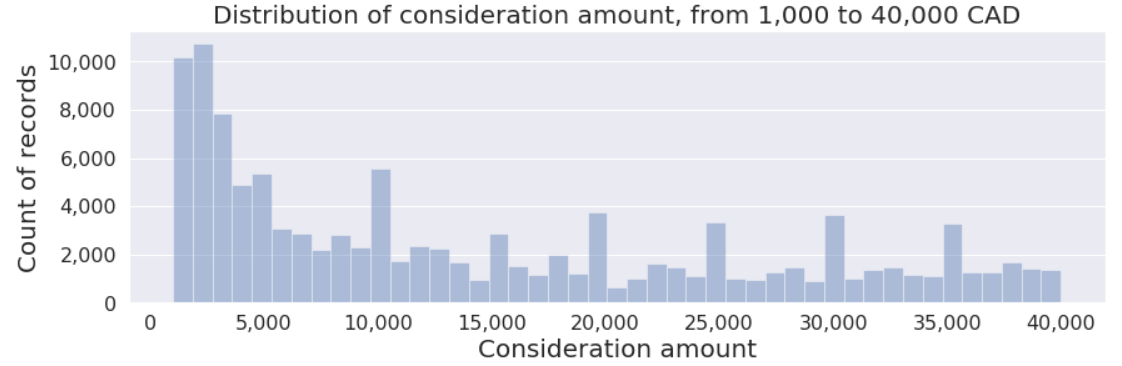
\includegraphics[width=.95\linewidth]{price_dist_zoom.png}
        \caption{From 1,000 to 40,000 CAD}
    \end{subfigure}
    \caption{Outliers at the bottom end of the price distribution most likely represent gift transactions.
    Since no clear break can be identified, 10,000 CAD was used as the bottom cut-off threshold for consideration amount to filter Teranet records.}
    \label{fig:bottom_outliers}
\end{figure}

In terms of transaction price distribution, outliers at both the high and the low end are present in Teranet's dataset:
\begin{itemize}
    \item There is a high number of transactions with very low consideration amounts (starting from a few dollars, shown on figure~\ref{fig:bottom_outliers}) that most likely represent transactions recording gifts of property, where some symbolic consideration amount has been used.
    \item At the same time, since Teranet's dataset includes sales of all categories of properties, some records have significantly higher consideration amounts that can range in the hundreds of millions and billions of dollars;
    these records most likely correspond to sales of large commercial and industrial properties or whole residential buildings.
\end{itemize}

Since low outliers represent transactions that are not useful for analysis, they were removed from the dataset.
However, there seems to be no way to establish what constitutes a reasonable bottom cut-off threshold, as there was no criteria available on how to define a gift transaction;
furthermore, no clear break could be identified on the low end of the price distribution.
Since there seems to be an exceptionally large spike of transactions with consideration amount under 10,000 CAD, they were considered to be low outliers and were removed from Teranet's dataset, further reducing the number of records from 6,803,691 to 5,188,513.

In case of outliers at the high end of the price distribution, they most likely correspond to transactions of expensive commercial and industrial property or whole residential buildings.
Since these transactions are useful for research questions concerning commercial and industrial property, they were left in the dataset and instead have been marked with special new attributes ``outlier'' using different criteria.
Since, again, there was no clear criteria available as to what would constitute a top outlier, instead of using a single criterion, seven different Boolean variables were added describing whether a record belongs to outliers according to a particular condition or not.
For example, feature `outlier\_y\_10' is a Boolean variable capturing if the price of a record, corrected for inflation, is over 10 times greater than the median price of all records for the corresponding year.
Table~\ref{tab:outliers} presents the outlier categories that were used and the count of Teranet records that each of them marked to belong to outliers.

\begin{table}[h!]
    \centering
    \begin{tabular}{|| c | c ||}
        \hline
        Category & Count of records \\
        \hline
        \hline
        outlier\_y\_3 & 251,537 \\
        \hline
        outlier\_y\_5 & 137,814 \\
        \hline
        outlier\_y\_10 & 84,260 \\
        \hline
        outlier\_y\_20 & 53,866 \\
        \hline
        outlier\_xy\_2 & 160,662 \\
        \hline
        outlier\_xy\_4 & 57,766 \\
        \hline
        outlier\_xy\_10: & 35,778 \\
        \hline
    \end{tabular}
    \caption{Categories of outliers and the count of Teranet records that were marked by them.
    For categories coded `y', price of each record was compared to median price of all Teranet records for that year;
    for categories coded `xy', prices were compared to median price of all records for that coordinate pair;
    a number represents the threshold that the ratio needed to exceed for a record to be considered an outlier.}
    \label{tab:outliers}

\end{table}

These new ``outlier'' attributes were used when filtering records during the assignment of reduced land use classes, which will be discussed in section~\ref{sec:select_encode_target};
in addition, they were tested as a part of the original full feature set for classification of land use along with the other new features engineered from Teranet's dataset, which will be discussed in section~\ref{sec:feature_engineering}.
However, in the case of classification, all of the new ``outlier'' features were filtered out in the process of feature selection;
feature selection will be discussed in section~\ref{sec:dimensionality_reduction}.
Instead, algorithms performed better with features that numerically represent price, such as 'med\_price\_xy', computed as the median consideration amount (in 2016 dollars) for a coordinate pair.

Some of the new features that have been engineered from original Teranet attributes, which will be discussed in section~\ref{sec:feature_engineering}, also contain outliers on the high end of their distributions.
For example, in the case of the feature `xy\_prev\_sales' which captures the rolling count of Teranet records from a coordinate pair, counts of records from a coordinate pair that corresponds to a house would be in the order of $10^1$, while counts of records from a coordinate pair that corresponds to an apartment building would be on the order of $10^2-10^4$.
In these cases, outliers contain valuable information that can be used to classify Teranet records by property type, but these outliers still present a challenge for the convergence of gradient-based algorithms.
To keep these records in the dataset while facilitating faster convergence, feature scaling was performed and will be discussed in section~\ref{sec:feature_scaling}.

\section{Engineering new features for the classification algorithm} \label{sec:feature_engineering}

In addition to producing new keys for joining datasets, a number of the new features was engineered from original Teranet attributes to be tested with classification algorithms (discussed in chapters~\ref{ch:ml_workflow} and~\ref{ch:model_evaluation}).
These new features were intended to give each Teranet record spatial and temporal ``context'' of the housing market dynamics by grouping records using different criteria.
For example, feature `xy\_prev\_sales' was computed as the rolling count of Teranet records coming from a particular coordinate pair;
feature `price\_to\_med\_year' captures the ratio of consideration amount of a record to the median consideration amount of all Teranet records for the corresponding year, etc.

The following features have been added to each Teranet record from 1985 to 2017 (`xy' represents `x' and `y' coordinates concatenated together as strings, used to group together all records coming from a particular coordinate pair):

\begin{itemize}
    \item `price\_2016': consideration amount (in 2016 dollars) using the coefficients from the Inflation Calculator provided by the Bank of Canada\cite{BankofCanada2019}
    \item `pin\_total\_sales': count of Teranet records grouped by `pin'
    \item `xy\_total\_sales': count of Teranet records grouped by `xy'
    \item `pin\_prev\_sales': rolling count of Teranet records grouped by `pin'
    \item `xy\_prev\_sales': rolling count of Teranet records grouped by `xy'
    \item `xy\_first\_sale': a Boolean variable indicating whether it is the first record coming from this `xy'
    \item `pin\_years\_since\_last\_sale': difference in years since the last record coming from this `pin'
    \item `xy\_years\_since\_last\_sale': difference in years since the last record coming from this `xy'
    \item `xy\_years\_to\_next\_sale': difference in years to the next record coming from this `xy'
    \item `da\_days/years\_since\_last\_sale': difference in days/years since the last sale that occurred on this Dissemination Area
    \item `xy\_sale\_next\_6m': a Boolean variable indicating whether there will be another sale on this `xy' in the upcoming 6 month
    \item `pin\_price\_cum\_sum': cumulative sum of price (in 2016 dollars) for all Teranet records coming from this `pin'
    \item `xy\_price\_cum\_sum': cumulative sum of price (in 2016 dollars) for all Teranet records coming from this `xy'
    \item `pin\_price\_pct\_change': percentage change of price (in 2016 dollars) from the last Teranet record from this `pin'
    \item `xy\_price\_pct\_change': percentage change of price (in 2016 dollars) from the last Teranet record from this `xy'
    \item `price\_da\_pct\_change': percentage change of price (in 2016 dollars) from the last Teranet record from this Dissemination Area
    \item `med\_price\_xy': median price (in 2016 dollars) for all Teranet records from this `xy'
    \item `med\_price\_year': median price (in 2016 dollars) for all Teranet records for this year
    \item `price\_to\_med\_xy': ratio of price (in 2016 dollars) to the median price of all records for this `xy'
    \item `price\_to\_med\_year': ratio of price (in 2016 dollars) to the median price of all records for this year
    \item `outlier\_y\_3': a Boolean variable marking as outliers all records with the price more than 3 times greater than median for that year
    \item `outlier\_y\_5': a Boolean variable marking as outliers all records with the price more than 5 times greater than median for that year
    \item `outlier\_y\_10': a Boolean variable marking as outliers all records with the price more than 10 times greater than median for that year
    \item `outlier\_y\_20': a Boolean variable marking as outliers all records with the price more than 20 times greater than median for that year
    \item `outlier\_xy\_2': a Boolean variable marking as outliers all records with the price more than 2 times greater than median for that `xy'
    \item `outlier\_xy\_4': a Boolean variable marking as outliers all records with the price more than 4 times greater than median for that `xy'
    \item `outlier\_xy\_10': a Boolean variable marking as outliers all records with the price more than 10 times greater than median for that `xy'
\end{itemize}

These new features were combined with TTS and Census variables via spatial and temporal relationships that were introduced in chapter~\ref{ch:spatial_and_temporal_relationships} and were used to train and test a classification algorithm to classify land use at Teranet transaction level, which is discussed in chapter~\ref{ch:ml_workflow}.

Some of the new engineered features, such as `xy\_years\_since\_last\_sale' and `xy\_years\_to\_next\_sale' contain missing values in each case of the first or the last Teranet record coming from a coordinate pair.
Since classification algorithms cannot handle inputs with missing values, during classification these values have been replaced with the corresponding median, which will be discussed in section~\ref{sec:missing_values}.
The recorded version of Teranet's dataset with the new features and keys would still have them as missing.

\section{Chapter summary} \label{sec:data_preparation_summary}

The principles of ``Tidy data'', closely related to Codd's principles of database normalization, formalize the way how a shape of the data can be described and what goal should be pursued when formatting data.
The ``tidy data'' standard  facilitates initial exploration and analysis of the data and simplifies the development of data analysis tools that work well together.
The structure of Teranet's dataset conforms with the ``Tidy data'' format.
Contrary to Teranet, tables with select Census and TTS variables had variables for different Census and TTS years recorded as columns and thus needed to be unpivoted.
A new attribute `year' was introduced to these tables to be used as a part of a composite foreign key when joining with Teranet records.

New foreign keys representing spatial identifiers, such as `dauid' and `taz\_o', were added to Teranet records via a series of spatial joins.
During the first join with Dissemination Area geometry used by Census, Teranet records with coordinates falling outside of GTHA have been filtered out.
Furthermore, Teranet records with consideration amount under 10,000 CAD were considered to be outliers at the low end of price distribution and were removed from the dataset.
Outliers at the high end of the price distribution were not removed, but instead were marked by seven new Boolean attributes using various criteria to define a top outlier.
Finally, new features have been engineered to be tested with classification algorithms, which will be described in chapters~\ref{ch:ml_workflow} and~\ref{ch:model_evaluation}.
In addition, datasets with new keys and features have been loaded into a PostgreSQL database established using referential integrity constraints based on the spatial and temporal relationships that were introduced in chapter~\ref{ch:spatial_and_temporal_relationships}.
